\chapter{Background}
\label{chap:background}

\begin{figure}
  \centering
  \begin{subfigure}{\textwidth}
    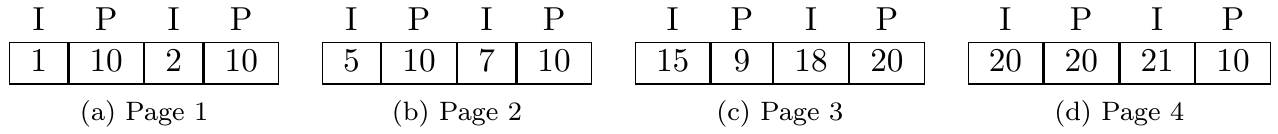
\includegraphics[width=\textwidth]{img/row-store.png}
    \caption{Row store layout.}
    \label{fig:row-column-store-1} 
  \end{subfigure}
  \begin{subfigure}{\textwidth}
    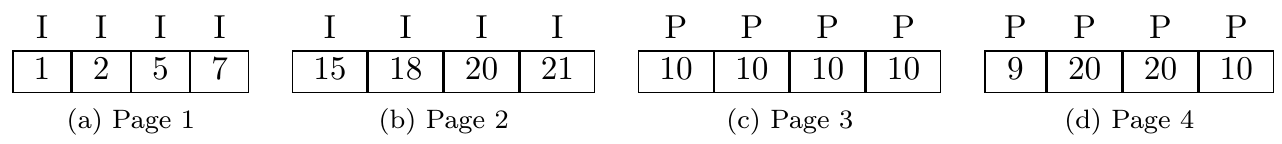
\includegraphics[width=\textwidth]{img/column-store.png}
    \caption{Column store layout.}
    \label{fig:row-column-store-2} 
  \end{subfigure}
  \caption{Row and column oriented layouts for a table with two columns, I and P. In the row-oriented layout (a), records (I and P tuples) are stored next to each other within the pages. In the column-oriented layout (b), values from the I column and P column are stored separately on different pages. Courtesy of \cite{Bjorklund2011-wh}.}
  \label{fig:row-column-store} 
\end{figure}
\section{Column Storage}
\label{sec:Column Storage}


The most common storage format for OLTP systems is row storage, as we briefly mentioned in Section \ref{sec:Definitions}. Row storage enables easy fetching of values from the same tuple, and is suited for updates, inserts, and deletes. However for OLAP workloads, columnar storage has turned out advantageous, mainly because of two reasons: First, aggregations are easier, since calculations are performed on data consecutive in memory. Second, column storage does not fetch more data than is needed for the query.

Our research has identified several systems using columnar storage. These include \monetdb~\cite{Boncz2005-wj, Boncz2002-yj}, \cstore~\cite{Stonebraker2005-qz}, \saph~\cite{Farber2012-vh}, and \mssql~\cite{noauthor_undated-vq, Larson2013-mc}, as well as the \bd~product \tableau~\cite{Kamkolkar2015-iq}.

In a column store, each column in a table is stored separately in a continuous segment (unless data is horizontally partitioned, see Section \ref{sec:Horizontal Partitioning}), as opposed to row stores where attributes from a single row are stored together \cite{Bjorklund2011-wh}. Figure \ref{fig:row-column-store} depicts both row and column oriented layouts for a table with two columns (I and P). The row storage alternates between I and P to store records next to each other on the pages while the column storage keeps I and P values separate. 

The advantages of using column storage are many. The primary one is that no more data is accessed than strictly necessary for a query. In addition to this, columns are inherently more compressible \cite{noauthor_undated-vq}. Compression leads to higher performance due to better cache and memory utilization, and this effect is one of the reasons why \mssql~use column storage. We elaborate on the performance benefits of compression in Chapter \ref{chap:Data Compression}.

Column storage also comes with a more subtle advantage; columns have a \textit{low degree of freedom} compared to row storage \cite{Boncz2005-wj}. When operating on column values, only the local memory offset is required, not the global table layout. This removes some layers of indirection and query processing can be made more efficient. Boncz \ea~claim that this is the main reason why column storage is advantageous.


One of the major disadvantages with column store is that it is not as easily updateable \cite{Bjorklund2011-wh}, especially if the columns are compressed or sorted. This challenge is normally overcome using a separate structure for writes and updates called a \textit{delta store}. Using such structure, the main part of the database is stored column-wise in a static structure optimized for reads while the updates and inserts are accumulated in a smaller and more dynamic structure. We investigate delta stores further in Section \ref{sub:Delta Store}.

Another disadvantage with column storage is tuple materialization costs. Since the result of most DBMS queries should be returned as rows, columns must be stitched back together before returned to the client, an operation that can be expensive.


\subsection{Sorting}
\label{sub:Sorting}
We see that few systems sort the data values before storing them to columns. An exception to this is \cstore, and later \vertica~\cite{Lamb2012-kg, Stonebraker2005-qz}. In these systems, \textit{column projections} can be defined, which is a subset of the columns in a table. Each column projection is sorted based on one column in the subset, which means a column is either sorted by own values or by values from another column in the projection. Projections are specified by the database administrator. A column can have multiple projections, hence multiple sort orders, which results in data duplication. The extra storage needed for multiple column sort orders is justified by the compression that column storage enables.


Sorting values in a column store comes with some advantages. First, single value lookups are easily performed by a binary search (however, this limitation can be overcome by keeping inverted indexes \cite{Lemke2010-is, Schwalb2014-hn}, which we study in Section \ref{sec:Inverted Indexes}) Second, and perhaps most important, is that sorted columns can be compressed aggressively by applying \rle. \rle~is the main reason \cstore~stores sorted data \cite{Stonebraker2005-qz}. We study this type of compression in Section \ref{sec:Run-Length Encoding}.

Column sorting also comes with a performance benefit. Holloway \ea~show how sorted columns perform better due to \rle~\cite{Holloway2008-rr}. \blink~has also reported a performance increase if the columns are sorted prior to testing \cite{Johnson2008-cp}, even if this system does not use \rle.

Except from \cstore~and \vertica, our research has shown little indication that sorting values in columns are common. For instance, \mssql~\cite{Larson2013-mc}, \blink~\cite{Raman2013-em} and \oracle~\cite{Lahiri2015-mz} accept values in the order they appear.

Although most systems do not sort values in the columns and instead accept values as they arrive, many systems have a sorted dictionary when \de~is used. Systems here include \blink~\cite{Johnson2008-cp} and \saph~\cite{Farber2012-vh}. A sorted dictionary has many advantages, like easy lookup for single values, transformation of range predicates to \texttt{IN}-list predicates, and partition pruning. A sorted dictionary structure is better suited for a read-only environment, since updating a sorted dictionary requires some work. We look into \de~in Section \ref{sec:Dictionary Encoding}.

\subsection{Row Stores vs Column Stores}
\label{sub:Row Stores vs Column Stores}
Most research agree that row stores are most suitable for OLTP workloads, and column stores are most suitable for OLAP workloads. Abadi \ea~set out to investigate whether there is a fundamental difference between row and column stores \cite{Abadi2008-dd}. In their research, they used a row store with a vertically partitioned schema to mimic a colum store. They also tried applying indexes to each column such that each column could be accessed independently. Their conclusion was that there \textit{is something fundamental about column stores} that makes them perform so well, and that changes must be made to both storage layer and query executor to obtain the benefits of a column-oriented approach. The main reasons why column storage is better suited for OLAP workloads are:
\begin{itemize}
  \item \textit{Compression}, which we discuss in Chapter \ref{chap:Data Compression}.
  \item \textit{Vectorized execution}, which we discuss in Section \ref{sec:Loop Pipelining and Vectorized Execution}.
  \item \textit{Late materialization}, which we discuss in Section \ref{sec:Late Materialization}.
\end{itemize}

There are situations for OLAP databases where a row store performs better than a column store. A research executed by Holloway \ea~shows that a row store can outperform a column store when processing time is the dominating contraint \cite{Holloway2008-rr}. This is typically the case for low selectivity queries and queries with many predicates. To further improve row storage performance, tuples can be compressed. However, row storage will most likely never beat column stores for OLAP workloads, since bandwidth requirement for processing rows is higher than for columns.

\ffigure{img/chain-reaction.png}{OLTP workloads will affect more than a couple of rows. Index structures must be maintained, and aggregations and materialized views must be updated. In the figure, an update that triggers a chain reaction is depicted. Courtesy of \cite{Plattner2014-fr}.}{fig:chain-reaction}

We have also identified papers that claim OLTP databases also benefit from a columnar storage. The work of Farber \ea~argues that columnar storage is suited for transactional workloads as well, mainly due to the compression \cite{Farber2012-vh}. Also, storing data in columns allows for dropping indexes, which is normally costly to maintain. Last, there are normally a lot more read operations than inserts, updates, and deletes in an OLTP database.

Plattner \ea~claim that most OLTP queries request aggregates instead of single rows \cite{Plattner2014-fr}. In addition, updates to the database normally triggers a chain reaction of updates to indexes and materialized views, as seen in Figure \ref{fig:chain-reaction}. Their conclusion is that column storage is suited for OLTP databases due to efficient aggregation and abscence of indexes. The absence of indexes also makes application development easier, since no performance layer must be specified by the application programmer.

We have earlier in this chapter said that columns are more compressible than rows. However, the work of Holloway \ea~claims that row stores can be compressed just as much if done correctly \cite{Holloway2008-rr}. We believe that even though rows are as compressible as columns, compression of columns is simpler and more practical.

\subsection{Row Identifiers and Tuple Materialization}
\label{sub:Row Identifiers and Tuple Materialization}
A row in a column store is identified by a unique identifier that is common to every value belonging to the same row in a table. Many systems store these IDs implicitly as virtual object IDs (\texttt{void}). A \texttt{void} for an object is calculated using a base ID and the offset from the first value in the column. For instance, the fourth value of a column with base ID 100 has an implicit ID of 103. \texttt{void} type identifiers are used in \monetdb~\cite{Boncz2002-yj}, \cstore~\cite{Stonebraker2005-qz}, \vertica~\cite{Lamb2012-kg}, and \ibm~\cite{Raman2013-em}.

If horizontal partitioning is used, a technique we discuss in the next section, the partition number must also be accounted for in row identification. For instance, \mssql~identifies a row by a combination of row group ID and tuple ID \cite{Larson2013-mc}.

For systems that do not keep columns sorted, stitching together rows is pretty straight forward. All columns selected in a query can be iterated in order and tuples can be materialized before sent back to the client. Needless to say, the operation of stitching together rows comes at a higher cost in a column store than for a row store.

Stitching together columns with different sort orders is a very expensive operation. \cstore~uses join indexes for this operation, which we study in Section \ref{sec:Join Indexes}. \vertica~only allows a query to access columns belonging to the same projection. In other words, a query must use a projection that contains all the columns needed for the query.

\section{Bitpacking}
\label{sec:Bitpacking}

\afigure{img/bitpacking.png}{Bitpacked column values. Values are stored with no more bits than needed to represent the column, which results in values that are not aligned to machine word boundaries. Values may be spread across several machine words and share their machine word(s) with other codewords. Courtesy of \cite{Willhalm2013-ri}.}{fig:bitpacking}{0.8}

\bp~is a trivial form of compression, where values are stored with no more bits than needed. In other words, if a column has a cardinality of 32, only 5 bits are required to represent a value. This way, in a 32-bit architecture, 100 values can be stored using $500$ bits, and not $100*32 = 3200$. \bp~has lower compression than algorithms that allow variable length for values, but values can be randomly accessed in constant time \cite{Raman2008-gi, Willhalm2013-ri}. Also, \bp~enables SIMD processing, which we discuss in Section \ref{sec:SIMD}. \bp~is well suited for high cardinality, uniform distribution of values, where dictionary encoding only provides an unnecessary layer of indirection \cite{Holloway2008-rr}.

As seen in Figure \ref{fig:bitpacking}, bitpacked values will not generally align to word boundaries. For processing, values normally have to be moved to the word boundary, but this cost has been found to be negligible \cite{Holloway2008-rr}. Aligning values can be done in an SIMD like fashion, a technique we study in Section \ref{sec:SIMD}.

In its simplest form, \bp~works directly on the column data, but the compression scheme can be more powerful if combined with other compression types. We see in Section \ref{sec:Dictionary Encoding} that dictionary keys can be bitpacked, and in Section \ref{sec:Delta Encoding} that \dele~benefits from \bp~if the deltas between the values are small. Besides, bitpacked vectors can be used in an inverted index structure \cite{Schwalb2014-hn}, which we study in Section \ref{sec:Inverted Indexes}.

\subsection{Issues with Bitpacking}
\label{sub:Issues with Bitpacking}
\afigure{img/partitioned-bitpack.png}{A normal bitpacked vector (left) and a partitioned bitpacked vector (right). Instead of rebuilding the entire vector on value overflow, the partitioned bitpacked vector has different partitions where each partition is compressed using an increasing number of bits. Courtesy of \cite{Faust2015-ke}.}{fig:partitioned-bitpack}{0.9}
There are two major limitations with \bp~\cite{Faust2015-ke}. The first is that if the bitpacking overflows, the full bitpacked vector must be rebuilt. What this means is that if all values are mapped, such that there are no available values with $n$ bits, a new bit must be introduced, and the entire vector must be rebuilt where each value has $n + 1$ bits. This is depicted in the left part of Figure \ref{fig:partitioned-bitpack}. To counter this effect, Faust \ea~have suggested a partitioned bitpacked vector structure that creates a new partition with $n + 1$ bits on overflow, as seen in the right part of Figure \ref{fig:partitioned-bitpack}. Although this technique improves performance on insert operations, read performance suffers due to the extra overhead of looking up a value.

The second limitation with \bp~is that it does not account very well for data skew. In \bp, each distinct value in a vector contributes to the total number of bits required, completely disregarding the distribution of the values. Often in a database, there are a large number of distinct values, but they are not uniformly distributed. This problem can be solved with the partitioned vectors explained in the previous paragraph, by mapping the values that occur more frequently to the partitions with the fewest bit per value. Other algorithms map outliers to a separate structure, like \pfdelta~\cite{Bjorklund2011-wh}.


\section{Dictionary Encoding}
\label{sec:Dictionary Encoding}
\de, or \term{Dictionary Compression}, is widely used within column store databases. Systems that use \de~include \oracle~\cite{Lahiri2015-mz}, \ibm~\cite{Raman2013-em}, \saph~\cite{Farber2012-vh}, \sapnw~\cite{Lemke2010-is}, \blink~\cite{Johnson2008-cp}, \mssql~\cite{Larson2013-mc}, and more. \qlikview~stores each distinct data point only once \cite{Qlik2011-ef}. \tableau~does not mention anything about \de~in their whitepapers, but an official blog post claims that this compression technique is used \cite{noauthor_undated-us}.

\afigure{img/dictionary-sorted.png}{A sorted dictionary. Each distinct value is stored only once in the dictionary. A key is assigned to each entry in the dictionary, and those keys are stored in the columns instead of the actual values. Courtesy of \cite{Psaroudakis2014-ma}.}{fig:dictionary-sorted}{0.4}

In a dictionary encoded column, each distinct value is stored once in a structure known as \textit{the dictionary}. Keys are assigned to each entry in the dictionary, most commonly integers from zero and up. Columns store these keys and not the actual values, and data is compressed since each unique value is stored exactly once. \de~using a sorted dictionary is illustrated in Figure \ref{fig:dictionary-sorted}. \de~is particularly effective when a column in a column store has only a few distinct values in a large dataset \cite{Faust2015-ke}.


Except from the compression, one of the major advantages of \de, is that many database operations can be performed directly on the encoded values \cite{Faust2015-ke}, which we have seen in Section \ref{sub:Working Directly on Compressed Data} is important to achieve good performance. Integer comparison are less expensive than comparing the actual values, especially for strings. Additionally, range and \texttt{LIKE} predicates can be turned into \texttt{IN}-list operations, since the dictionary can be scanned first to find the relevant integer keys \cite{Barber2012-xt}.

If the columns are partitioned horizontally, which we have discussed in Section \ref{sec:Horizontal Partitioning}, it is common that each partition has a separate dictionary. This is the case for most database systems, like \oracle~\cite{Lahiri2015-mz}, \blink~\cite{Barber2012-xt}, and \mssql~\cite{Larson2013-mc}. When a dictionary is stored per partition, it can be used for quick data pruning; if a value is not present in the dictionary, the partition can be skipped. \blink~and \monetx~use this technique \cite{Barber2012-xt, Boncz2005-wj}. 

When implementing \de, special considerations should be taken. First, if the dictionary turns out bigger than the values it is replacing, \de~should not be used \cite{Holloway2008-rr}. Secondly, \de~performs best if the dictionary fits inside the L2 cache of a processor.

Like \bp, \de~does not handle data skew very well, since each unique value needs an entry in the dictionary no matter how frequent that value appears in a column. Besides, for high cardinality columns, the compression is less efficient.

\subsection{Sorted Dictionaries}
\label{sub:Sorted Dictionaries}
Dictionaries can be either sorted or unsorted. Using a sorted dictionary enables easier value lookup using a binary search. However, more important for us, is that using a sorted dictionary can turn range scans into simple integer comparisons \cite{Faust2015-ke}. For instance, if we want to find all sales in 2010, we only need to look up the integer codes for January 1st, 2010 and January 1st, 2011 and find all integers within this range. Since integer comparisons are fast and effective, this technique will usually improve performance. 

Most database systems today use sorted dictionaries. \saph~is an example of such system \cite{Farber2012-vh}.

However, as briefly mentioned in Section \ref{sub:Sorting}, keeping a dictionary sorted implies a higher overhead on database inserts, updates and deletes. We see in Section \ref{sub:Delta Store} that some systems divide their data into two stores: A read-optimized store, and a delta store (for updates and inserts). With this division, it is common to use a sorted dictionary for the read-optimized store and an unsorted dictionary for the delta store \cite{Plattner2014-fr}.

\subsection{Dictionary Encoding and Bitpacking}
\label{sub:Dictionary Encoding and Bitpacking}
\de~is commonly used in conjunction with \bp. With this combination, the dictionary keys in the columns are stored with no more bits than necessary. Since dictionary keys normally are integers from zero to the number of entries, bitpacking enables high compression rates, especially for low-cardinality columns.

Systems using \de~and \bp~include \ibm~\cite{Raman2013-em}, \blink~\cite{Barber2012-xt}, \sapnw~\cite{Willhalm2009-hu}, and \saph~\cite{Psaroudakis2014-ma}. \qlikview~has also reported to compress data with only the number of bits required \cite{Qlik2014-vd}. \mssql~does not apply \bp~on dictionary keys in columns, and instead store them as 32-bit integers \cite{Larson2013-mc}.

The same advantages and disadvantages of \bp~apply to \de~with bitpacked columns. For instance, values can be looked up in constant time and queries can be processed in an SIMD-like fashion. However, insertions to the dictionary might lead to an overflow, which requires the entire column to be rebuilt.

\section{Background Information on Modern CPUs and Compilers}
\label{sec:Background Information on Modern CPUs and Compilers}
Modern processors are capable of performing an enormous amount of calculations per second, but that depends on the amount of available and independent work. The instructions-per-second (IPC) difference between minimal and maximal CPU utilization can easily be one order of magnitude \cite{Boncz2005-wj}. Hence, database software must be implemented such that it fully exploits the processing power made available by the CPU.

\subsection{Pipelining, Superscalar Processing, and Independent Instructions}
\label{sub:Pipelining, Superscalar Processing, and Independent Instructions}
\afigure{img/superscalar.png}{A simple superscalar pipeline. Multiple execution units allow for processing multiple instructions in parallel. Courtesy of \cite{Wikipedia_contributors2015-kp}.}{fig:superscalar}{0.6} 

Modern processors improve clock rate and IPC by using a technique known as \textit{pipelining} \cite{Boncz2005-wj}. By dividing an instruction execution into multiple steps, there is less work per stage, and the CPU frequency can be increased. Figure \ref{fig:superscalar} depicts an example pipeline with five stages. However, pipelining also introduce two dangers; \textit{instruction dependencies} and \textit{branch misprediction}.

In a pipeline, \textit{dependencies between instructions} impose a problem. If an instruction is dependent on another, it must wait for the other instruction to complete before it enters the pipeline. Dependent instructions can severely hurt performance, especially if the pipeline is long.

Conditional branches are also affected by dependencies between instructions. When executing a conditional branch instruction, the decision whether to take a branch is usually dependent on the result of a preceding instruction \cite{Boncz2005-wj}. To avoid stalling the pipeline when waiting for the expression to evaluate, modern CPUs use a technique known as branch prediction where the processor immaturely starts executing the branch that is most likely to be taken. The performance penalty occurs if a branch is \textit{mispredicted}, where the instructions in the pipeline must be invalidated (pipeline flushing).

Another way that performance is increased in a processor is by having muliple execution units. We refer to such processors as \textit{superscalar}. As seen in Figure \ref{fig:superscalar}, a superscalar processor can have multiple instructions in the same stage of the pipeline, which allows IPC (instructions per cycle) $> 1$. However, for this functionality to be fully utilized, independent work is required.

\begin{figure}
  \centering
  \begin{subfigure}{0.45\textwidth}
    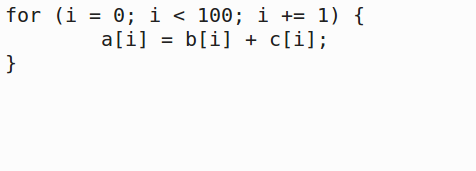
\includegraphics[width=\textwidth]{img/loop-unrolling-1.png}
    \caption{Original loop}
    \label{fig:loop-unrolling-1} 
  \end{subfigure}
  \begin{subfigure}{0.45\textwidth}
    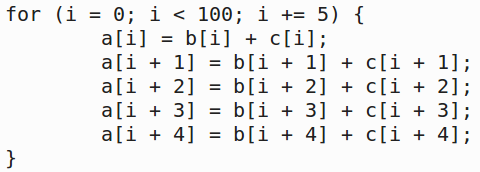
\includegraphics[width=\textwidth]{img/loop-unrolling-2.png}
    \caption{Unrolled loop}
    \label{fig:loop-unrolling-2} 
  \end{subfigure}
  \caption{By unrolling loops, instructions are made independent and the number of branches is reduced.}
  \label{fig:loop-unrolling} 
\end{figure}
Hence, to reach maximum performance for a pipelined, superscalar processor, we must find independent work. Since most programming languages do not let the programmer specify which instructions are independent of each other, compiler optimizations play a critical role in CPU utilization \cite{Boncz2005-wj}. The most widely used technique used by the compilers to address this challenge is \textit{loop unrolling}, which is used to reduce the number of branches and increase independence between instructions \cite{Wikipedia_contributors2015-zc}. As seen in Figure \ref{fig:loop-unrolling}, loop unrolling reduces the number of iterations in a loop (reduction of branches) and replaces it with multiple instances of the same instruction. If the instructions are independent, they can be processed in parallel.

\subsection{CPU Caches}
\label{sub:CPU Caches}
Since transfering data from main memory to CPU can take around $~200$ cycles, modern CPUs utilize multiple layers of on- and off-chip caches to reduce this latency. Efficient usage of caches is paramount for CPU throughput, since roughly 30\% of all instructions in a program are memory loads or stores \cite{Boncz2005-wj}. We know that IPC for DBMSes is strongly impaired by cache misses, and cache utilization is an important topic for in-memory databases \cite{Exasol2014-xh}.

The best way to tackle this challenge is to design algorithms and data structures that are \textit{cache aware} \cite{Farber2012-vh}. Designing such programs is out of the scope of this report, but it briefly boils down to two things:
\begin{itemize}
  \item \textit{Coordinate temporal and spatial locality}. Data processed together should be stored at consecutive memory addresses. Code locality is also important \cite{Neumann2011-uq}.
  \item \textit{Avoid false sharing of cache lines}. Multiple cores in a processor should not write to data belonging to the same cache entry at the same time to avoid unecessary invalidations.
\end{itemize}
\textit{Compression}, which we described in Chapter \ref{chap:Data Compression}, and \textit{vectorized execution}, which we discuss in Section \ref{sec:Loop Pipelining and Vectorized Execution}, are two techniques used to improve cache performance \cite{Larson2013-mc, Lemke2010-is}.

\textit{Prefetching} is another method used to increase cache utilization. Prefetching proactively loads data into caches such that the data is available when an instruction needs it.

\subsection{Call Stack and Subroutine Invocations}
\label{sub:Call Stack and Subroutine Invocations}
\afigure{img/call-stack.png}{A call stack for a program in execution. Each stack frame contains input parameters, function return address, and local variables for a subroutine invocation. Courtesy of \cite{Wikipedia_contributors2015-od}.}{fig:call-stack}{0.5}

A \textit{call stack} is commonly used in a computer program to store information and state about active subroutines \cite{Wikipedia_contributors2015-od}. Each time a subroutine is called, a \textit{stack frame} is added to the call stack that stores the input arguments, return address, and variables local to the subroutine. See Figure \ref{fig:call-stack}. The call stack can be implemented in both hardware and software, and the implementation varies between different systems. This stack-based technique implies that calling a subroutine comes at a cost; registers must be stored on the stack, and a new stack frame must be added.

Trading off time with space is usually done to address the above challenge; adding more code to improve program efficiency. \textit{Function inlining} is a technique used by compilers where the subroutine code is copied into the caller's body. This way, no new stack frame is created for the subroutine, avoiding the overhead associated with a function invocation.

\textit{Macro expansion} is another form of code generation. Macros are normally specified by the application programmer, and can be used for programmer-controlled inlining of functions or constant values. Macros can also be used to generate multiple versions of function or class definitions (templating), a technique commonly used to let a single implementation support different data types.

\section{Branch Avoidance}
\label{sec:Branch Avoidance}
\ffigure{img/branch-selectivity.png}{Predicate evaluation performance for queries with different query selectivities. A \textit{branch version} and a \textit{predicated version} are tested. For the AthlonMP processor, the branch version are 2-3 times slower on queries with 40\%-60\% selectivity, while the Itanium2 processor has constant processing time. The predicated version offers constant processing time for both processors. Courtesy of \cite{Boncz2005-wj}.}{fig:branch-selectivity}

We saw in the previous section that branches should be avoided due to the penalties of branch misprediction. Besides, branches also cause dependencies between instructions. 

The consequences of inaccurate branch prediction are studied by Neumann \ea~\cite{Neumann2011-uq}. In this research, the performance of queries with various selectivities was tested. As we can see in Figure \ref{fig:branch-selectivity}, queries with 40\%-60\% selectivity executed on an AthlonMP processor are roughly 2-3 times slower than queries with selectivities close to 0\% or 100\%. Hence, selectivity can severely affect the query performance. The Itanium2 processor does not have the same characteristic, as the Itanium architecture allows for both \textit{not taken} and \textit{taken} branches to be executed simultaneously.

Neumann \ea~also developed a branchless version (predicated version) to evaluate predicates in the queries. The branchless variant is denoted as \texttt{predicated version} in Figure \ref{fig:branch-selectivity}. For both AthlonMP and Itanium2 processors, this implementation offers constant performance for all selectivities, but is, in general, more expensive.

Branch avoidance is also important in other parts of the system, for instance when decompressing. Zukowski \ea~present a decompression algorithm that is free for \textit{if-then-else} statements \cite{Zukowski2006-oz}. By running the algorithm in two tight loops instead of one, branch misprediction is reduced, and the loops can be pipelined by a compiler.

Branches can also be avoided by compiling queries to machine code \cite{Lamb2012-kg}. We will elaborate on this technique in Section \ref{sub:Compiling Queries to Machine Code}.

\subsection{Short-Circuiting}
\label{sub:Short-Circuiting}
\begin{figure}
  \centering
  \begin{subfigure}{0.45\textwidth}
    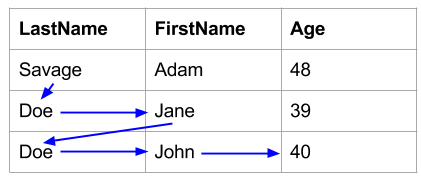
\includegraphics[width=\textwidth]{img/short-circuiting-1.png}
    \caption{Short-circuiting}
    \label{fig:short-circuiting-1} 
  \end{subfigure}
  \begin{subfigure}{0.45\textwidth}
    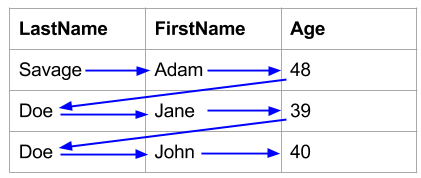
\includegraphics[width=\textwidth]{img/short-circuiting-2.png}
    \caption{No short-circuiting}
    \label{fig:short-circuiting-2} 
  \end{subfigure}
  \caption{Predicate evaluation for query \texttt{WHERE LastName='Doe' AND FirstName='John' AND Age>21}. (a) skips evaluating rest of the predicates if one predicate is false, while (b) evaluates all predicates regardless of previous results.}
  \label{fig:short-circuiting} 
\end{figure}
\textit{Short-circuiting} is referred to a special case of Boolean operator evaluation in which the next argument is not evaluated if the current argument is sufficient to determine the value of the expression \cite{Wikipedia_contributors2015-rk}. Figure \ref{fig:short-circuiting} illustrates the difference between short-circuit and non-short-circuit predicate evaluation. In short-circuiting, the scan proceeds to the next tuple as soon as one predicate is false, as opposed to the verision without short-circuiting that evaluates all predicates regardless of previous results.

Since short-circuit boolean operators are control structures and not simple arithmetic operators, there is a chance of branch misprediction. That is why \blink~does not short-circuit between tuples \cite{Raman2008-gi, Johnson2008-cp}. If a block is selected for scanning, all fields in the records are checked. According to Raman \ea, short-circuiting only improves performance on low selectivity queries \cite{Raman2008-gi}.

\section{\mdd}
\label{sec:mdd}
Model-driven development is defined as *.

\mendix, one of the market players in \mdd, uses a JavaScript blabla.

We investigate \genusSoftware in the following chapter.


